\chapter{Implementierung des DDQN-Ansatzes}
\label{chap:implementierung}

Dieses Kapitel beschreibt, wie der in Abschnitt~\ref{sec:ansatz_vergleich} gewählte Double-DQN-Agent (DDQN) in PyTorch umgesetzt ist. Die Implementierung besteht aus drei Teilen: einer Gymnasium-Umgebung, die Netzwerkflüsse als Merkmalsvektoren erzeugt und über einen AWGN-Kanal stört, dem DDQN-Agenten mit Replay-Puffer und Zielnetz sowie einer vektorisierten Trainingsschleife, die standardmäßig auf einer CUDA-GPU läuft. Alle Größen stammen aus dem Quelltext (\texttt{train\_eval.py}).

\section{Systemarchitektur und Gesamtüberblick}
\label{sec:systemarchitektur}

Jeder Netzwerkfluss ist eine eigene, unabhängige Entscheidung. Der Agent erhält einen verrauschten Merkmalsvektor, wählt \emph{Normal} oder \emph{DDoS} und bekommt sofort eine Belohnung. Der Folgefluss hängt weder von der Aktion noch vom aktuellen Fluss ab. Eine Episode umfasst deshalb genau einen Schritt (\texttt{terminated=True}). Die Pipeline lässt sich in vier Stufen gliedern:

\begin{enumerate}
	\item \textbf{Flussgenerator:} Aus dem Modell in Abschnitt~\ref{sec:generatormodell} entsteht pro Fluss ein Vektor $\mathbf{x}\in\mathbb{R}^8$ samt Label.
	\item \textbf{AWGN-Kanal:} Auf $\mathbf{x}$ wird additives Rauschen entsprechend dem SNR addiert, der Agent sieht $\mathbf{y}$.
	\item \textbf{DDQN-Agent:} Ein Q-Netz bewertet beide Aktionen, die Aktion mit dem größten Q-Wert (bzw. eine $\epsilon$-greedy-Aktion) wird ausgeführt.
	\item \textbf{Lernschritt:} Die Transition wird im Replay-Puffer gespeichert, aus dem Mini-Batches das Online-Netz trainieren.
\end{enumerate}

Abbildung~\ref{fig:blockschaltbild} zeigt die Wirkungskette vom Flussgenerator bis zur Entscheidung. Der Rückpfad vom Reward in den Replay-Puffer schließt den Lernkreis, der Reward erreicht den Agenten also ausschließlich als Trainingssignal und nie als Eingabe.

\begin{figure}[htbp]
	\centering
	\begin{tikzpicture}[
		font=\small,
		blk/.style={draw, rectangle, rounded corners=2pt, minimum height=1.35cm, text width=2.7cm, align=center, thick},
		ch/.style={blk, fill=blue!8, text width=3.0cm},
		ag/.style={blk, fill=green!10},
		rw/.style={blk, fill=orange!12, text width=3.0cm},
		sub/.style={draw, rectangle, minimum height=0.5cm, text width=2.4cm, align=center, font=\scriptsize, fill=white},
		arr/.style={-{Stealth[length=2.2mm]}, thick}
	]
		% Umgebung: Generator, Kanal, Reward
		\node[blk] (gen) at (0,0) {Flussgenerator\\ {\scriptsize $\mathbf{x}\in\mathbb{R}^{8}$, Label $c$}};
		\node[ch] (awgn) at (4.4,0) {AWGN-Kanal\\ {\scriptsize $\sigma_{n,j}^{2}=P_j/10^{\mathrm{SNR}/10}$\\ SNR $30$ bis $5$\,dB}};
		\node[rw] (rew) at (11.4,0) {Reward-Matrix\\ {\scriptsize asymmetrisch, $r(a,c)$}};
		\draw[arr] (gen) -- node[above, font=\scriptsize] {$\mathbf{x}$} (awgn);
		\draw[arr] (gen.north) -- ++(0,0.45) -| node[pos=0.25, above, font=\scriptsize] {Label $c$} (rew.north);
		\begin{scope}[on background layer]
			\node[draw=black!55, dashed, rounded corners=3pt, fit=(gen)(awgn)(rew), inner xsep=0.25cm, inner ysep=0.95cm, yshift=0.4cm,
				label={[font=\scriptsize, black!70, anchor=north west, inner sep=2pt]north west:Gymnasium-Umgebung \texttt{DDoSFlowEnv}}] (gym) {};
		\end{scope}

		% Agent mit Innenleben
		\node[ag] (agent) at (4.4,-3.3) {DDQN-Agent\\ {\scriptsize $\epsilon$-greedy}};
		\node[sub, below=0.3cm of agent] (onl) {Online-Netz $\theta$};
		\node[sub, below=0.1cm of onl] (tgt) {Zielnetz $\bar\theta$};
		\node[sub, below=0.1cm of tgt] (rb) {Replay-Puffer};
		\begin{scope}[on background layer]
			\node[draw, dashed, fit=(agent)(onl)(tgt)(rb), inner sep=4pt, fill=green!5] (agbox) {};
		\end{scope}

		% Entscheidung
		\node[blk] (dec) at (11.4,-3.3) {Entscheidung\\ {\scriptsize $a\in\{0,1\}$}};

		\draw[arr] (awgn) -- node[pos=0.72, right, font=\scriptsize] {Beobachtung $\mathbf{y}$} (agbox.north);
		\draw[arr] (agent) -- node[above, font=\scriptsize] {$a$} (dec);
		\draw[arr] (dec) -- node[right, font=\scriptsize] {$a$} (rew);
		\draw[arr, dashed] (rew.east) -- ++(0.45,0) |- node[pos=0.75, below, font=\scriptsize] {Reward $r$} (rb.east);
	\end{tikzpicture}
	\caption[Blockschaltbild der Wirkungskette]{Blockschaltbild der Wirkungskette. Die Gymnasium-Umgebung (gestrichelter Rahmen) erzeugt $\mathbf{x}$ mit Label $c$, stört $\mathbf{x}$ über den AWGN-Kanal und bewertet die Entscheidung $a$ des Agenten über die Reward-Matrix gegen $c$. Der Reward $r$ gelangt nur als Trainingssignal in den Replay-Puffer (gestrichelter Pfeil), nie als Eingabe des Agenten.}
	\label{fig:blockschaltbild}
\end{figure}

Der Zustand ist direkt der Merkmalsvektor, der Aktionsraum hat zwei Elemente. Diese Vereinfachung hält die Umgebung schnell: Der Flussgenerator erzeugt 32 Flüsse pro Iteration vektorisiert in NumPy, und Puffer, Netze und Rewards liegen auf demselben Rechengerät (standardmäßig eine CUDA-GPU), sodass beim Sampling kein Transfer zwischen Host und Gerät anfällt.

\section{Gymnasium-Umgebung und Zustandsraum}
\label{sec:gymnasium_umgebung}

Die Klasse \texttt{DDoSFlowEnv} erbt von \texttt{gymnasium.Env} und definiert:

\begin{itemize}
	\item \textbf{Beobachtungsraum:} \texttt{Box}$(-\infty,\infty)^{8}$ vom Typ \texttt{float32}, der verrauschte Merkmalsvektor $\mathbf{y}$.
	\item \textbf{Aktionsraum:} \texttt{Discrete}$(2)$ mit $a=0$ (Normal) und $a=1$ (DDoS).
	\item \textbf{Reset:} zieht einen neuen Fluss mit Label $c\in\{0,1\}$ (Angriffsanteil $\pi=0{,}3$) beim fest eingestellten SNR der Umgebung.
	\item \textbf{Step:} berechnet den Reward aus Aktion und Label, liefert eine Null-Beobachtung und setzt \texttt{terminated=True}. Die Terminal-Beobachtung geht nicht in das Lernen ein.
\end{itemize}

Der Gymnasium-Umgebungsprüfer (\texttt{check\_env}) validiert die Schnittstelle vor jedem Lauf. Die Belohnung hängt allein vom Zusammenspiel von Aktion und wahrem Label ab:

\begin{equation}
	r(a,c)=
	\begin{cases}
		R_{\mathrm{TP}}=+1{,}0, & a=1,\ c=1 \\
		R_{\mathrm{TN}}=+0{,}5, & a=0,\ c=0 \\
		R_{\mathrm{FP}}=-1{,}0, & a=1,\ c=0 \\
		R_{\mathrm{FN}}=-2{,}0, & a=0,\ c=1 .
	\end{cases}
\end{equation}

Ein verpasster Angriff kostet doppelt so viel wie ein Fehlalarm. Diese Asymmetrie wirkt als kostensensitives Lernziel anstelle eines Resamplings (Abschnitt~\ref{sec:imbalanced_data}). Für die Evaluation in Kapitel~\ref{chap:ergebnisse} hat sie eine konkrete Folge, nämlich die Verschiebung der Soll-Schwelle auf $p>1/3$ (Abschnitt~\ref{sec:mdp_definition}).

\subsection{Formale Definition als Markov-Entscheidungsprozess}
\label{sec:mdp_definition}

Das Entscheidungsproblem ist ein Markov-Entscheidungsprozess $(\mathcal{S},\mathcal{A},\mathcal{P},\mathcal{R},\gamma)$ in der Notation von Sutton und Barto \autocite{suttonReinforcementLearningIntroduction2018} mit folgenden Komponenten:

\begin{itemize}
	\item \textbf{Zustandsraum:} $\mathcal{S}=\mathbb{R}^{8}$. Ein Zustand ist die verrauschte Beobachtung $\mathbf{y}=\mathbf{x}+\mathbf{n}$ mit $n_j\sim\mathcal{N}(0,\sigma_{n,j}^2)$ aus Abschnitt~\ref{sec:awgn_kanal}. Das Label $c$ gehört nicht zum Zustand, der Prozess ist bezüglich $c$ nur teilbeobachtbar.
	\item \textbf{Aktionsraum:} $\mathcal{A}=\{0,1\}$, mit $a=0$ für Normalverkehr und $a=1$ für DDoS.
	\item \textbf{Transition:} $\mathcal{P}(\mathbf{y}'\mid\mathbf{y},a)$ ist deterministisch und von $(\mathbf{y},a)$ unabhängig. Jede Episode endet nach einem Schritt, das Terminal-Flag ist stets $d=1$:
	\begin{equation}
		\mathcal{P}(\mathbf{y}'\mid\mathbf{y},a)=\delta(\mathbf{y}'-\mathbf{0}),\qquad d=1 .
	\end{equation}
	Der Folgezustand ist die Null-Beobachtung aus \texttt{step}. Der nächste Fluss entsteht erst im \texttt{reset}. Im vektorisierten Training speichert der Replay-Puffer als Folgebeobachtung stattdessen die aktuelle Beobachtung $\mathbf{y}$. Wegen $d=1$ geht dieser Wert in keines der Lernziele ein.
	\item \textbf{Belohnung:} $\mathcal{R}(a,c)$ als Reward-Matrix mit Zeilen $c$ und Spalten $a$:
	\begin{equation}
		\mathcal{R}=
		\begin{pmatrix}
			\mathcal{R}(0,0) & \mathcal{R}(1,0)\\
			\mathcal{R}(0,1) & \mathcal{R}(1,1)
		\end{pmatrix}
		=
		\begin{pmatrix}
			R_{\mathrm{TN}} & R_{\mathrm{FP}}\\
			R_{\mathrm{FN}} & R_{\mathrm{TP}}
		\end{pmatrix}
		=
		\begin{pmatrix}
			+0{,}5 & -1{,}0\\
			-2{,}0 & +1{,}0
		\end{pmatrix}.
	\end{equation}
	Das entspricht \texttt{REWARD\_TABLE[label, action]} im Quelltext.
	\item \textbf{Diskontierung:} $\gamma=0{,}99$. Wegen $d=1$ geht $\gamma$ nicht in das Ziel ein.
\end{itemize}

Die optimale Politik maximiert den erwarteten Sofort-Reward $\mathbb{E}[\mathcal{R}(a,c)\mid\mathbf{y}]$. Mit $p=P(c=1\mid\mathbf{y})$ gilt $a=1$ genau dann, wenn $p\,R_{\mathrm{TP}}+(1-p)\,R_{\mathrm{FP}}>p\,R_{\mathrm{FN}}+(1-p)\,R_{\mathrm{TN}}$, also $p>1/3$. Elkans Schwelle $p^*=(c_{10}-c_{00})/(c_{10}-c_{00}+c_{01}-c_{11})$ liefert mit den negierten Rewards als Kosten denselben Wert \autocite{elkanFoundationsCostSensitiveLearning2001}. Das ist die Soll-Schwelle, wenn das Q-Netz die bedingten Erwartungswerte des Rewards lernt. Der im Training verwendete Huber-Verlust verschiebt sie auf $3/7$ (Abschnitt~\ref{sec:dqn_architektur}), gemessen entscheidet der Agent bei impliziten Schwellen von $0{,}38$ bis $0{,}43$ (Abschnitt~\ref{sec:reward_recall}).

Im Training werden die Flüsse nicht einzeln über \texttt{step} erzeugt, sondern als Batch von 32 Flüssen pro Iteration, wobei das SNR jedes Flusses zufällig aus $\{30,20,10,5\}$\,dB gezogen wird. Der Rewardvektor entsteht durch eine Tabellenabfrage \texttt{REWARD\_TABLE[label, action]} direkt auf dem Rechengerät.

\section{DDQN-Architektur in PyTorch}
\label{sec:dqn_architektur}

Das Q-Netz (\texttt{QNet}) ist ein vollständig verbundenes Netz mit zwei verdeckten Schichten:
\begin{equation}
	\mathbb{R}^{8}\ \to\ \underbrace{128}_{\text{ReLU}}\ \to\ \underbrace{128}_{\text{ReLU}}\ \to\ \mathbb{R}^{2}.
\end{equation}
Abbildung~\ref{fig:qnet_architektur} stellt die Struktur dar. Mit Gewichtsmatrizen $\mathbf{W}_1\in\mathbb{R}^{128\times8}$, $\mathbf{W}_2\in\mathbb{R}^{128\times128}$, $\mathbf{W}_3\in\mathbb{R}^{2\times128}$ und Biasvektoren $\mathbf{b}_i$ berechnet das Netz
\begin{equation}
	\mathbf{q}(\mathbf{y})=\mathbf{W}_3\,\mathrm{ReLU}\!\bigl(\mathbf{W}_2\,\mathrm{ReLU}(\mathbf{W}_1\mathbf{y}+\mathbf{b}_1)+\mathbf{b}_2\bigr)+\mathbf{b}_3 .
\end{equation}
Die Parameterzahl beträgt $(8\cdot128+128)+(128\cdot128+128)+(128\cdot2+2)=17\,922$ je Netz.

\begin{figure}[htbp]
	\centering
	\begin{tikzpicture}[
		font=\small,
		lay/.style={draw, rectangle, rounded corners=2pt, minimum height=2.2cm, minimum width=1.5cm, align=center, thick},
		arr/.style={-{Stealth[length=2.2mm]}, thick},
		node distance=1.3cm
	]
		\node[lay, fill=gray!10] (in) {Eingabe\\ $\mathbf{y}\in\mathbb{R}^{8}$};
		\node[lay, fill=blue!10, right=of in] (h1) {Linear\\ $8\to128$\\ ReLU};
		\node[lay, fill=blue!10, right=of h1] (h2) {Linear\\ $128\to128$\\ ReLU};
		\node[lay, fill=green!10, right=of h2] (out) {Linear\\ $128\to2$};
		\node[right=1.0cm of out, align=left] (q) {$Q(\mathbf{y},0)$\\[2pt] $Q(\mathbf{y},1)$};
		\draw[arr] (in) -- (h1);
		\draw[arr] (h1) -- (h2);
		\draw[arr] (h2) -- (out);
		\draw[arr] (out) -- (q);
	\end{tikzpicture}
	\caption[Feedforward-Struktur des Q-Netzes]{Feedforward-Struktur des Q-Netzes ($8\to128\to128\to2$, ReLU in beiden verdeckten Schichten, lineare Ausgabe). Online- und Zielnetz teilen sich diese Struktur.}
	\label{fig:qnet_architektur}
\end{figure}

Die Ausgabeschicht ist linear, die zwei Ausgaben sind die Q-Werte $Q(\mathbf{y},0)$ und $Q(\mathbf{y},1)$. Online-Netz und Zielnetz haben dieselbe Struktur, das Zielnetz startet mit den Gewichten des Online-Netzes und wird nur kopiert, nie per Gradient trainiert. Zielnetz und Replay-Puffer gehen auf den DQN-Ansatz von Mnih et al. zurück, wo sie die Korrelation aufeinanderfolgender Transitionen aufbrechen und das Regressionsziel zwischen zwei Synchronisationen festhalten \autocite{mnihHumanlevelControlDeep2015}.

Im Standard-DQN wählt und bewertet dasselbe Zielnetz die Folgeaktion:
\begin{equation}
	Y^{\mathrm{DQN}} = r + \gamma\,(1-d)\,\max_{a'} Q(\mathbf{y}',a';\bar{\theta}).
\end{equation}
Sind die Q-Schätzungen verrauscht, greift der $\max$-Operator bevorzugt Aktionen mit positivem Schätzfehler heraus, und das Ziel überschätzt den wahren Wert systematisch. Das DDQN-Ziel nach van Hasselt et al. trennt deshalb Aktionsauswahl und Bewertung \autocite{vanhasseltDeepReinforcementLearning2016}:
\begin{equation}
	Y = r + \gamma\,(1-d)\;Q\!\left(\mathbf{y}',\ \arg\max_{a'} Q(\mathbf{y}',a';\theta);\ \bar{\theta}\right),
\end{equation}
wobei $\theta$ die Parameter des Online-Netzes, $\bar\theta$ die des Zielnetzes und $d\in\{0,1\}$ das Terminal-Flag sind. Der Verlust ist die Huber-Funktion (\texttt{smooth\_l1\_loss}) zwischen $Q(\mathbf{y},a;\theta)$ und $Y$, die Gradientennorm wird auf $10$ begrenzt.

Weil jede Episode nach einem Schritt endet, gilt für alle gespeicherten Transitionen $d=1$ und damit $Y=r$. Abbildung~\ref{fig:backup} stellt den allgemeinen Fall und diesen Spezialfall als Backup-Diagramme gegenüber. Das Bootstrapping-Glied entfällt, der Diskontierungsfaktor $\gamma$ beeinflusst das Lernen nicht, und das Q-Netz regressiert den Sofort-Reward je Aktion (ein kontextuelles Banditenproblem). Online-/Zielnetz, Double-Q-Ziel und Replay-Puffer sind vollständig implementiert und bleiben im Code aktiv. Unter diesem Problemzuschnitt geht das Zielnetz wegen $d=1$ jedoch nie in $Y$ ein. Die Überschätzung, gegen die van Hasselt et al. das Double-Q-Ziel entwickelt haben, entsteht erst im Bootstrapping-Glied und kann hier nicht auftreten. Wirksam bleiben der Replay-Puffer, der die Mini-Batches dekorreliert, und die Huber-Regression auf den Sofort-Reward. Das ist bei der Interpretation der Ergebnisse zu berücksichtigen.

Der Huber-Verlust hat dabei eine Nebenwirkung auf die Entscheidungsschwelle. Er ist für Residuen $|Y-Q|\le1$ quadratisch und darüber linear. Die Rewards einer Aktion liegen aber $2$ (Aktion DDoS: $+1$ oder $-1$) bzw. $2{,}5$ (Aktion Normal: $-2$ oder $+0{,}5$) auseinander. Das Minimum des erwarteten Verlusts liegt deshalb nicht beim bedingten Erwartungswert, sondern zwischen Erwartungswert und Median. Für $p<1/2$ ergibt die Stationaritätsbedingung $Q_{\mathrm{H}}(\mathbf{y},1)=(2p-1)/(1-p)$ und $Q_{\mathrm{H}}(\mathbf{y},0)=0{,}5-p/(1-p)$, für $p>1/2$ entsprechend $(2p-1)/p$ und $(1-p)/p-2$. Daraus folgt
\begin{equation}
	Q_{\mathrm{H}}(\mathbf{y},1)-Q_{\mathrm{H}}(\mathbf{y},0)=
	\begin{cases}
		\dfrac{3{,}5\,p-1{,}5}{1-p}, & p<1/2,\\[8pt]
		\dfrac{5\,p-2}{p}, & p>1/2,
	\end{cases}
\end{equation}
mit der Nullstelle $p=3/7\approx0{,}43$ statt $1/3$. Ein mit diesem Verlust trainiertes Q-Netz entscheidet also konservativer, als die Reward-Matrix vorgibt. Abschnitt~\ref{sec:reward_recall} prüft das am trainierten Netz.

\begin{figure}[htbp]
	\centering
	\begin{tikzpicture}[
		font=\small,
		st/.style={circle, draw, thick, minimum size=4.4mm, inner sep=0pt},
		ac/.style={circle, fill, minimum size=2.3mm, inner sep=0pt},
		te/.style={rectangle, fill, minimum size=2.8mm, inner sep=0pt},
		gst/.style={circle, draw=black!35, dashed, thick, minimum size=4.4mm, inner sep=0pt},
		gac/.style={circle, fill=black!30, minimum size=2.3mm, inner sep=0pt},
		ed/.style={thick},
		ged/.style={draw=black!35, dashed, thick}
	]
		% (a) allgemeiner Fall
		\begin{scope}
			\node[ac, label={[font=\scriptsize]above:$(s,a)$}] (sa) at (0,0) {};
			\node[st] (s1) at (0,-1.25) {};
			\node[font=\scriptsize, right=1.5mm of s1] {$s'$};
			\draw[ed] (sa) -- node[left, font=\scriptsize] {$r$} (s1);
			\foreach \x/\n in {-0.75/a1, 0/a2, 0.75/a3} { \node[ac] (\n) at (\x,-2.45) {}; \draw[ed] (s1) -- (\n); }
			\draw[thick] ($(s1)!0.42!(a1)$) to[bend right=35] ($(s1)!0.42!(a3)$);
			\node[font=\scriptsize, anchor=east] at ($(s1)!0.42!(a1)+(-0.05,0)$) {$\max$};
			\node[font=\scriptsize, below=1mm of a2] {$a'$};
			\node[font=\scriptsize, right=1.5mm of a3, align=left] {wählt: Online-Netz $\theta$\\ bewertet: Zielnetz $\bar\theta$};
			\node[font=\scriptsize] at (0.6,-3.3) {$Y=r+\gamma\,(1-d)\,Q\bigl(s',\arg\max_{a'}Q(s',a';\theta);\bar\theta\bigr)$};
			\node at (0.6,-3.95) {(a) allgemeiner Fall ($d=0$)};
		\end{scope}
		% (b) Ein-Schritt-Episode dieser Arbeit
		\begin{scope}[xshift=8.4cm]
			\node[ac, label={[font=\scriptsize]above:$(\mathbf{y},a)$}] (ya) at (0,0) {};
			\node[te] (T) at (0,-1.25) {};
			\node[font=\scriptsize, right=1.5mm of T] {Terminalzustand, $d=1$};
			\draw[ed] (ya) -- node[left, font=\scriptsize] {$r$} (T);
			\node[gst] (g1) at (0,-1.95) {};
			\draw[ged] (T) -- (g1);
			\foreach \x/\n in {-0.6/b1, 0/b2, 0.6/b3} { \node[gac] (\n) at (\x,-2.75) {}; \draw[ged] (g1) -- (\n); }
			\node[font=\scriptsize, text=black!55, right=1.5mm of b3, align=left] {Bootstrapping-Zweig\\ entfällt: $\gamma\,(1-d)=0$};
			\node[font=\scriptsize] at (0.6,-3.3) {$Y=r$};
			\node at (0.6,-3.95) {(b) diese Arbeit (Ein-Schritt-Episode)};
		\end{scope}
	\end{tikzpicture}
	\caption[Backup-Diagramme des Lernziels]{Backup-Diagramme des Lernziels in der Notation von Sutton und Barto \autocite{suttonReinforcementLearningIntroduction2018} (offener Kreis: Zustand, Punkt: Aktion, Quadrat: Terminalzustand). (a) Im allgemeinen Fall bootstrappt das Double-DQN-Ziel über den Folgezustand $s'$: Das Online-Netz wählt $a'$, das Zielnetz bewertet sie. (b) In dieser Arbeit endet jede Episode nach einem Schritt. Der Bootstrapping-Zweig (grau) entfällt, das Ziel reduziert sich auf $Y=r$, und Zielnetz und Double-Q-Ziel gehen nicht in das Lernen ein.}
	\label{fig:backup}
\end{figure}

Der Replay-Puffer (\texttt{ReplayBuffer}) ist ein Ringpuffer mit $50\,000$ Einträgen nach dem Schema von Mnih et al. \autocite{mnihHumanlevelControlDeep2015}. Er hält Beobachtung, Aktion, Reward, Folgebeobachtung und Terminal-Flag als Tensoren auf dem Zielgerät und zieht gleichverteilte Mini-Batches der Größe $64$.

\section{AWGN-Kanalmodell im Lernprozess}
\label{sec:awgn_kanal}

Der Agent beobachtet $\mathbf{y}=\mathbf{x}+\mathbf{n}$ mit $n_j\sim\mathcal{N}(0,\sigma_{n,j}^2)$ je Merkmal $j$. Das ist das AWGN-Kanalmodell der Nachrichtentechnik \autocite{proakisDigitalCommunications2008}, hier nicht auf ein Sendesignal, sondern auf den Merkmalsvektor angewendet (Abschnitt~\ref{sec:merkmalsrauschen}). Die Rauschvarianz richtet sich nach der Signalleistung $P_j=\mathbb{E}[x_j^2]$ des Merkmals und dem gewünschten SNR (Abschnitt~\ref{sec:generatormodell}):
\begin{equation}
	\sigma_{n,j}^2=\frac{P_j}{10^{\mathrm{SNR_{dB}}/10}}.
\end{equation}
Der Kanalfaktor ist $h=1$, es gibt keine Verstärkung oder Fading-Komponente. Bei $30$\,dB beträgt die Rauschvarianz $10^{-3}P_j$, bei $5$\,dB etwa $0{,}32\,P_j$. Die Rauschstandardabweichung beträgt damit etwa $3\,\%$ (bei $30$\,dB) bis $56\,\%$ (bei $5$\,dB) von $\sqrt{P_j}$. Bei $5$\,dB liegt die Rauschstandardabweichung mit $0{,}22$ bis $0{,}31$ je Merkmal über der intrinsischen Klassenstreuung $\sigma=0{,}20$.

\subsection{Klassenüberlappung bei sinkendem SNR}
\label{sec:klassenueberlappung}

Das Rauschen verbreitert beide Klassenverteilungen. Die Beobachtung ist klassenbedingt wieder gaußverteilt, denn die Summe zweier unabhängiger Gauß-Terme bleibt gaußförmig:
\begin{equation}
	y_j\mid c\sim\mathcal{N}\!\bigl(\mu_{c,j},\ \sigma^2+\sigma_{n,j}^2\bigr).
\end{equation}
Die Klassenmittelwerte bleiben fest, nur die Varianz wächst von $\sigma^2=0{,}04$ auf $\sigma^2+\sigma_{n,j}^2$. Der Abstand der Mittelwerte $\Delta\mu_j=\mu_{\text{DDoS},j}-\mu_{\text{Normal},j}$ beträgt $\pm0{,}15$ bis $\pm0{,}25$. Bei gleicher Kovarianz beider Klassen (diagonal) ergibt sich der Mahalanobis-Abstand
\begin{equation}
	D^{2}=\sum_{j=1}^{8}\frac{\Delta\mu_j^{2}}{\sigma^{2}+\sigma_{n,j}^{2}},
\end{equation}
und die Bayes-Fehlerwahrscheinlichkeit für gleiche Priors ist $P_e=Q_{\mathrm{G}}(D/2)$ mit der Gaußschen Q-Funktion
\begin{equation}
	Q_{\mathrm{G}}(z)=\frac{1}{\sqrt{2\pi}}\int_{z}^{\infty}e^{-t^{2}/2}\,\mathrm{d}t .
\end{equation}
Der Index G trennt sie von der Aktionswertfunktion $Q(\mathbf{y},a)$ des Agenten. Der Zusammenhang entspricht der Symbolfehlerwahrscheinlichkeit binärer Signale im AWGN-Kanal, bei der $D$ die Rolle des normierten Signalabstands übernimmt \autocite{proakisDigitalCommunications2008}. Mit dem tatsächlichen Angriffsanteil $\pi=0{,}3$ verschiebt die Bayes-Regel ihre Schwelle um $\lambda=\ln\bigl((1-\pi)/\pi\bigr)$ auf der Skala des Log-Likelihood-Verhältnisses, und die minimale Fehlerwahrscheinlichkeit lautet
\begin{equation}
	P_e^{\pi}=\pi\,Q_{\mathrm{G}}\!\left(\frac{D}{2}-\frac{\lambda}{D}\right)+(1-\pi)\,Q_{\mathrm{G}}\!\left(\frac{D}{2}+\frac{\lambda}{D}\right).
\end{equation}
Für die Parameter aus \texttt{train\_eval.py} liefert die Auswertung die Werte in Tabelle~\ref{tab:klassenueberlappung}.

\begin{table}[htbp]
	\centering
	\renewcommand{\arraystretch}{1.25}
	\caption[Klassenseparierbarkeit der Beobachtung in Abhängigkeit vom SNR]{Klassenseparierbarkeit der Beobachtung $\mathbf{y}$ in Abhängigkeit vom SNR ($\sigma=0{,}20$). $P_e$: Bayes-Fehler bei gleichen Priors, $P_e^{\pi}$: Bayes-Fehler beim tatsächlichen Angriffsanteil $\pi=0{,}3$.}
	\label{tab:klassenueberlappung}
	\begin{tabular}{rrrrrr}
		\toprule
		\textbf{SNR in dB} & $\max_j\sigma_{n,j}$ & $D^{2}$ & $D$ & $P_e=Q_{\mathrm{G}}(D/2)$ & $P_e^{\pi}$ \\
		\midrule
		$30$ & $0{,}018$ & $8{,}76$ & $2{,}96$ & $6{,}9\,\%$ & $6{,}2\,\%$ \\
		$20$ & $0{,}056$ & $8{,}33$ & $2{,}89$ & $7{,}4\,\%$ & $6{,}6\,\%$ \\
		$10$ & $0{,}176$ & $5{,}62$ & $2{,}37$ & $11{,}8\,\%$ & $10{,}4\,\%$ \\
		$5$  & $0{,}312$ & $3{,}17$ & $1{,}78$ & $18{,}7\,\%$ & $16{,}2\,\%$ \\
		\bottomrule
	\end{tabular}
\end{table}

Zwischen $30$ und $20$\,dB ändert sich die Überlappung kaum, weil das Rauschen ($\sigma_{n,j}\le0{,}056$) neben $\sigma=0{,}20$ vernachlässigbar bleibt. Bei $5$\,dB sinkt $D$ auf $1{,}78$, die effektive Streuung steigt je nach Merkmal auf $0{,}30$ bis $0{,}37$, und die Fehlerwahrscheinlichkeit des Bayes-Klassifikators steigt gegenüber $30$\,dB auf fast das Dreifache. Beim tatsächlichen Angriffsanteil $\pi=0{,}3$ liegt sie auf jeder Stufe etwas niedriger, von $6{,}2\,\%$ bei $30$\,dB bis $16{,}2\,\%$ bei $5$\,dB. Diese Spalte ist die Referenz für alle weiteren Vergleiche mit der Bayes-Grenze. Das Training mit gemischtem SNR zwingt das Q-Netz auf eine Kompromiss-Entscheidungsgrenze, die für kein SNR exakt optimal ist.

Abbildung~\ref{fig:llr_signalraum} zeigt dieselbe Rechnung als Signalraumdarstellung auf der Prüfgröße $\Lambda(\mathbf{y})=\ln\bigl(p(\mathbf{y}\mid\mathrm{DDoS})/p(\mathbf{y}\mid\mathrm{Normal})\bigr)$. Sie bündelt wie bei binären Signalen im AWGN-Kanal die gesamte Klasseninformation der acht Merkmale \autocite{proakisDigitalCommunications2008}. Bei der fehlerminimalen Schwelle $\tau(1/2)=\lambda$ ergeben beide Fehlerflächen zusammen genau $P_e^{\pi}$: bei $30$\,dB $3{,}5\,\%$ verpasste Angriffe und $2{,}7\,\%$ Fehlalarme, bei $5$\,dB $10{,}2$ und $6{,}0\,\%$, jeweils bezogen auf alle Flüsse. Die Soll-Schwelle $p>1/3$ der Reward-Matrix liegt um $\ln 2\approx0{,}69$ weiter links und tauscht verpasste Angriffe gegen Fehlalarme. Bei $5$\,dB sinkt der FN-Anteil auf $6{,}3\,\%$, der FP-Anteil steigt auf $11{,}5\,\%$. Der Gesamtfehler wächst dabei von $16{,}2$ auf $17{,}8\,\%$, die erwarteten Kosten unter der Reward-Matrix sinken.

\begin{figure}[htbp]
	\centering
	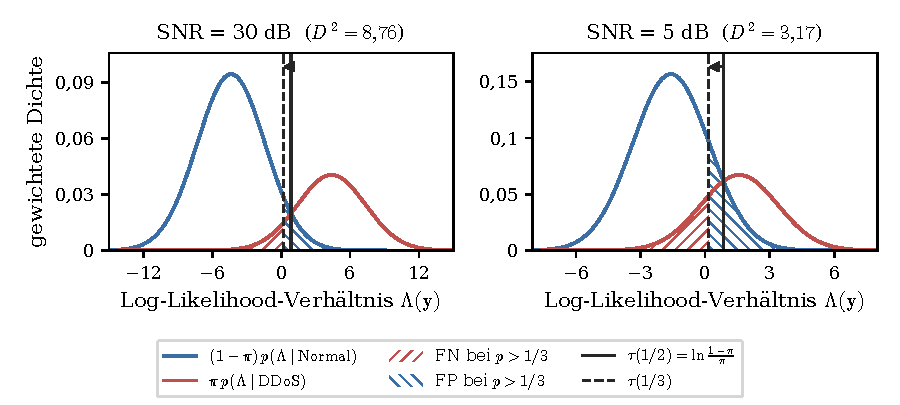
\includegraphics[width=\textwidth]{llr_signalraum_plot.pdf}
	\caption[Signalraumdarstellung auf dem Log-Likelihood-Verhältnis]{Signalraumdarstellung der binären Entscheidung auf der Prüfgröße $\Lambda(\mathbf{y})$ bei $30$ und $5$\,dB ($\pi=0{,}3$). Kurven: mit den Priors gewichtete Klassendichten $\pi\,\mathcal{N}(+D^2/2,D^2)$ und $(1-\pi)\,\mathcal{N}(-D^2/2,D^2)$. Durchgezogen: fehlerminimale Schwelle $\tau(1/2)=\lambda$, gestrichelt: Soll-Schwelle $\tau(1/3)$ der Reward-Matrix, Pfeil: Verschiebung um $\ln 2$. Schraffiert: Anteile verpasster Angriffe (FN) und Fehlalarme (FP) bei $p>1/3$.}
	\label{fig:llr_signalraum}
\end{figure}

Im Training trifft der Agent pro Fluss auf ein zufällig gewähltes SNR. Er lernt dadurch eine einzige Entscheidungsfunktion für alle vier Kanalqualitäten, ohne das SNR als Eingabe zu erhalten. Die Evaluation erfolgt dagegen getrennt je SNR-Stufe (Kapitel~\ref{chap:evaluierung}).

Das gemischte Training hat einen zweiten Effekt. Nach Bishop wirkt additives Eingangsrauschen im Training wie ein Tikhonov-Strafterm auf die Ableitungen der gelernten Abbildung (Abschnitt~\ref{sec:merkmalsrauschen}) \autocite{bishopTrainingNoiseEquivalent1995}. Das Q-Netz wird also gezwungen, $Q(\mathbf{y},a)$ glatt über $\mathbf{y}$ zu halten, und reagiert im Test weniger empfindlich auf einzelne Rauschausreißer. Apruzzese et al. nutzen dasselbe Prinzip mit gezielt gestörten Flussmerkmalen, um Detektoren gegen Evasion zu härten \autocite{apruzzeseDeepReinforcementAdversarial2020}. Streng gilt Bishops Äquivalenz nur für kleine Rauschvarianz. Bei $30$ und $20$\,dB ist diese Bedingung erfüllt ($\sigma_{n,j}\le0{,}056$), bei $5$\,dB mit $\sigma_{n,j}$ bis $0{,}31$ nicht mehr. Auf dieser Stufe bleibt die Regularisierungsdeutung eine qualitative Erklärung.

\section{Trainings- und Optimierungsstrategie}
\label{sec:training_optimierung}

Das Training läuft über $20\,000$ Iterationen. In jeder Iteration entstehen $32$ Flüsse, der Agent wählt $\epsilon$-greedy Aktionen, die Transitionen gelangen in den Puffer, und es folgt ein Lernschritt, sobald der Puffer mindestens $1000$ Einträge enthält. Die Explorationsrate fällt linear von $1{,}0$ auf $0{,}02$ innerhalb der ersten $40\,\%$ der Iterationen ($8000$) und bleibt danach konstant. Der Optimierer ist Adam mit Lernrate $10^{-4}$, der die Schrittweite je Gewicht aus gleitenden Schätzungen des ersten und zweiten Gradientenmoments anpasst \autocite{kingmaAdamMethodStochastic2015}. Das Zielnetz wird alle $250$ Lernschritte hart synchronisiert. Weil der Puffer je Iteration $32$ Transitionen aufnimmt, erreicht er die Mindestfüllung in Iteration $32$. Über den gesamten Lauf führt der Agent damit $19\,969$ Lernschritte mit je $64$ Transitionen aus und synchronisiert das Zielnetz $79$-mal. Ab Iteration $1563$ ist der Puffer voll, und neue Transitionen überschreiben die ältesten. Pro Seed (0, 1, 2) beginnt der Lauf mit neu initialisierten Netzen und eigenem Zufallsgenerator für die Flüsse. Die Seeds setzen Python-, NumPy- und PyTorch-Generatoren (inklusive CUDA).

\section{Implementierung in der praktischen Pipeline}
\label{sec:praktische_pipeline}

Das Skript \texttt{train\_eval.py} führt für jeden Seed Training und Evaluation aus und schreibt \texttt{evaluation\_results.csv} mit Precision, Recall und F1-Score je Seed und SNR sowie Mittelwert und Standardabweichung. Die Baselines (Random Forest, SVM, MLP) laufen in \texttt{eval\_baselines.py} und importieren Flussgenerator und Kanalmodell unverändert aus \texttt{train\_eval.py}. Dadurch sehen alle Verfahren dieselbe Datenverteilung und exakt dieselben Testflüsse. Die Abbildungen entstehen in \texttt{generate\_plot.py} aus den beiden CSV-Dateien.

Tabelle~\ref{tab:dqn_hyperparameters} fasst die Hyperparameter zusammen, Tabelle~\ref{tab:system_parameters} die Umgebungs- und Kanalparameter.

\begin{table}[htbp]
	\centering
	\renewcommand{\arraystretch}{1.25}
	\caption{Hyperparameter des DDQN-Agenten.}
	\label{tab:dqn_hyperparameters}
	\begin{tabular}{llL{6.2cm}}
		\toprule
		\textbf{Hyperparameter} & \textbf{Wert} & \textbf{Beschreibung} \\
		\midrule
		Netzstruktur & $8\to128\to128\to2$ & Zwei verdeckte Schichten mit ReLU \\
		Lernrate & $1\cdot10^{-4}$ & Adam-Optimierer \\
		Diskontierungsfaktor $\gamma$ & $0{,}99$ & Ohne Wirkung, da alle Episoden nach einem Schritt enden \\
		Batch-Größe & $64$ & Stichprobe pro Lernschritt \\
		Puffergröße & $50\,000$ & Ringpuffer auf dem Rechengerät \\
		Explorationsrate $\epsilon$ & $1{,}0 \to 0{,}02$ & Linear über $40\,\%$ der Iterationen \\
		Lernstart & $1000$ Einträge & Mindestfüllung des Puffers \\
		Zielnetz-Update & alle $250$ Lernschritte & Harte Synchronisation \\
		Verlustfunktion & Huber & Gradientennorm begrenzt auf $10$ \\
		Iterationen & $20\,000$ & Je $32$ Flüsse, insgesamt $6{,}4\cdot10^{5}$ Flüsse \\
		\bottomrule
	\end{tabular}

	\bigskip
	\renewcommand{\arraystretch}{1.25}
	\caption{System- und Kanalparameter der Simulationsumgebung.}
	\label{tab:system_parameters}
	\begin{tabular}{L{4.4cm}L{3.6cm}L{5.0cm}}
		\toprule
		\textbf{Parameter} & \textbf{Wert} & \textbf{Bedeutung} \\
		\midrule
		Zustandsraum & $\mathbb{R}^{8}$ & Verrauschter Merkmalsvektor $\mathbf{y}$ \\
		Aktionsraum & $2$ diskrete Aktionen & Normal (0), DDoS (1) \\
		Klassenstreuung $\sigma$ & $0{,}20$ & Je Merkmal, klassenbedingt gaußverteilt \\
		Angriffsanteil $\pi$ & $0{,}3$ & Klassenungleichgewicht \\
		Kanalmodell & AWGN, $h=1$ & Varianz $P_j/10^{\mathrm{SNR}/10}$ je Merkmal \\
		Evaluierte SNR-Werte & $30,\,20,\,10,\,5$\,dB & Abstufungen der Kanalqualität \\
		Reward\newline $(R_{\mathrm{TP}},R_{\mathrm{TN}},R_{\mathrm{FP}},R_{\mathrm{FN}})$ & $(+1;\,+0{,}5;\,-1;\,-2)$ & Asymmetrisch zulasten verpasster Angriffe \\
		Seeds & $0,\,1,\,2$ & Je ein vollständiger Trainings- und Testlauf \\
		Testflüsse & $20\,000$ je SNR und Seed & Frisch erzeugt, nicht im Training \\
		\bottomrule
	\end{tabular}
\end{table}

\section{Zusammenfassung der Implementierung}
\label{sec:implementierung_zusammenfassung}

Die Implementierung bildet die DDoS-Erkennung als Entscheidungsproblem mit acht verrauschten Merkmalen und zwei Aktionen ab, dessen Episoden nach einem Schritt enden. Das DDQN-Gerüst aus Online-Netz, Zielnetz, Double-Q-Ziel und Replay-Puffer ist vollständig umgesetzt. Die Kosten der Fehlerarten stecken in der Reward-Matrix, die Kanalqualität im AWGN-Modell mit SNR-Werten von $30$ bis $5$\,dB. Weil die Entscheidungen unabhängig sind, reduziert sich das Lernziel auf eine Huber-Regression des Sofort-Rewards. Kapitel~\ref{chap:ergebnisse} wertet die Läufe quantitativ aus.
